\documentclass[12pt,reqno]{amsart}
\usepackage{amsfonts,amssymb,amsmath,amsthm,
            amssymb,amsopn,amsxtra,amstext,amsbsy}
%% \usepackage[cp1251]{inputenc} % Coding
\usepackage{epsfig}
\usepackage{array}
\usepackage{url}
\usepackage{tikz}
\usetikzlibrary{shapes.geometric,fit}
\usepackage[spanish]{babel}
%\usepackage[latin1]{inputenc}
\usepackage[utf8x]{inputenc}
%% \usepackage{amsmath}
%% \usepackage{amsthm}
%% \usepackage{graphicx}
%% \usepackage{amsfonts}
\usepackage{color}
\usepackage{enumerate}
\newtheorem*{myteo}{Teorema}
\newtheorem*{mydef}{Definici\'on}

\voffset=-10mm
\oddsidemargin=0pt
\evensidemargin=0pt
\topmargin=-10mm
\headsep=10mm
\headheight=18pt
\footskip=30pt
\topskip=0mm
\textwidth 167mm
\textheight=230mm
\parindent=5mm
\marginparsep=3mm
\marginparwidth=19mm
\vfuzz2pt % Don't report over-full v-boxes if over-edge is small
\hfuzz6pt % Don't report over-full h-boxes if over-edge is small


%% MYREMARK ENVIRONMENT %%%%%%%%%%%
\newenvironment{mycolor}{\color{red}}{}
\newcounter{myremarkcount}
\setcounter{myremarkcount}{0}
\newsavebox{\myremarkbox}
\newenvironment{myremark}
{% This is the begin code
\medskip
\begin{flushright}
\begin{lrbox}{\myremarkbox}%
\begin{minipage}[t]{0.9\linewidth}
\stepcounter{myremarkcount}
\footnotesize
\begin{mycolor}
{\bf Remark \arabic{myremarkcount}.}
\begin{it}
}
{% This is the end code
\end{it}
\end{mycolor}
\end{minipage}
\end{lrbox}
\fbox{\usebox{\myremarkbox}}
\end{flushright}

\bigskip}



\title{Kernel Trick}
\author{Paola Arce \and Raquel Pezoa}

\begin{document}
\maketitle

\section{Idea Intuitiva de Kernels}
Supondremos que tenemos un conjunto con dos clases de objetos.
Al llegar un nuevo objeto, interesa saber a cu\'al de
las dos clases pertenece.
Este tipo de problema se denomina
{\bf problema de clasificaci\'on de objetos}. \cite{smola}.

Para poder realizar dicha clasificaci\'on en el contexto de m\'aquinas de
aprendizaje es necesario disponer de {\bf datos de entrenamiento}:

$$
(x_1,y_1),\,(x_2,y_2),\dots\,,\,(x_n,y_n)\ \in X\times\{-1,1\},
$$

\noindent donde $X$ es simplemente --por el momento-- un conjunto no vac\'\i o
y $x\in X$ corresponde al dato de entrada (tambi\'en denominados casos,
observaciones, patrones, etc.) e $y$ corresponde a la salida o etiqueta
asociada al dato de entrada.


Se espera que los algoritmos de m\'aquinas de  aprendizaje sean capaces de \emph{generalizar}, es decir,
los algoritmos deben predecir la etiqueta $y \in \{-1,1\}$
de los nuevos datos de entrada $x \in X$  mediante una funci\'on --o modelo-- constru\'ida
a partir de los datos de entrenamiento.
Para entender la idea, analicemos un ejemplo simple.
Supongamos que $X=\mathbb{R}$  y que los valores los valores de $x\in X=\mathbb{R}$ que son
mayores que $\pi$, por ejemplo, est\'an en la clase $y=+1$, y aquellos que son menores que $\pi$, est\'an en la clase $y=-1$.
Cuando el sistema recibe una entrada $x=\sqrt{11}$, \'este generaliza y responde que esta entrada pertenece a la clase $y=+1$.



La predicci\'on de la etiqueta $y\in\{-1,1\}$, debe ser de alguna manera
\textbf{similar} a los datos de entrenamiento $(x,y)$.
%
Para medir la similitud entre datos, se pueden usar diversas funciones.
En el caso de las etiquetas $y\in\{-1,1\}$, caracterizar la similitud es
simple, ya que s\'olo pueden ocurrir dos situaciones:
o bien las etiquetas son id\'enticas, por lo tanto similares,  o  bien son diferentes.
%Con esto queremos decir, por el momento en t\'erminos muy generales, que
%se escoge una etiqueta $y$ tal que $(x,y)$ es de alguna manera similar
%(parecido, cercano) a los datos de entrenamiento.



En el caso de los datos de entrada, la caracterizaci\'on de  su
similitud es un poco m\'as compleja, y es un aspecto central en el campo de
las llamadas m\'aquinas de aprendizaje.
Para poder definir la similitud entre $x,x'\in X$, comenzemos introduciendo una medida de similitud de la forma:
\begin{equation}
\begin{array}{rcl}
k: X\times X & \rightarrow & \mathbb{R} \\ 
    (x,x')   & \rightarrow & k(x,x')\;, \\
\end{array}
\end{equation}
donde $k$ es una funci\'on que recibe dos
par\'ametros, $x$ y $x'$, ambos pertenecientes al conjunto de entradas
$X$ y cuya salida es un valor real que caracteriza la similitud de ambos
par\'ametros.
Supondremos que $k$ es una funci\'on sim\'etrica,
es decir, $k(x,x')= k(x',x)$ para todo $x,x'\in X$.
Esta funci\'on $k$, {\em ser\'a\/} denominada {\bf kernel}.
Para comprender la forma general de los kernels, es necesario que
entendamos ciertos conceptos mat\'ematicos que estudiaremos en las siguientes
secciones,
as\'\i\ es que comenzaremos con un caso particular para llegar a entender su
forma general.


Una medida de similitud simple se podr\'ia definir mediante un \textbf{producto interno}
\footnote{Revisar en Sec. \ref{sec:def} la definici\'on de producto
interno a partir de formas hermitianas.}
(tambi\'en conocido como producto escalar o producto punto).

Por ejemplo, para los vectores $x,x'\in\mathbb{R}^n$, se define
el \textbf{producto interno can\'onico} de la siguiente manera:
\begin{equation}
\langle\mathbf{x},\mathbf{x'}\rangle
:= \sum \limits_{i=1}^{N} [\mathbf{x}]_i [\mathbf{x'}]_i 
\end{equation}
{\color{red} donde $[x]_i$, resp.  $[x']_i$, denota la $i$-\'esima
componente del vector $x\in\mathbb{R}^N$, resp.  $x'\in\mathbb{R}^N$.
Otro ejemplo de producto interno importante es:
\begin{equation*}
\langle f,g\rangle = \int_0^\infty f(t)\,\overline{g(t)}\;dt\,,\qquad
f,g\in C([0,1],\mathbb{C})\,,
\end{equation*}
donde $C([0,1],\mathbb{C})$ denota la clase de las funciones
continuas sobre el intervalo compacto $[0,1]$ con valores en
$\mathbb{C}$.
Obs\'ervese que $|\langle f,g\rangle|<\infty$ para todo
$f,g\in C([0,1],\mathbb{C})$.
{\bf ?`Por qu\'e?}}


\begin{myremark}
Aqu\'\i\ convendr\'\i a anotar los axiomas que debe satisfacer todo
producto interno.
{\bf Nota:}\ Estos axiomas se mencionan m\'as adelante en el texto.
\end{myremark}

\textcolor{blue}{Todav\'ia me falta llegar a decir: ``diremos que dos entradas
$x,x'\in X$ son similares cuando ...''}





\section{Espacios de Hilbert}

\textcolor{blue}{yo definir\'ia primero espacios de Banach.}

\begin{mydef}
Un producto interno $\langle\cdot,\cdot\rangle$ sobre un espacio vectorial
{\bf real} $X$ es una aplicaci\'on 
$\langle\cdot,\cdot\rangle:X\times X\to\mathbb{R}$,
que es lineal con respecto al primer y al segundo argumento
y es tal que 
$\langle\mathbf{x}, \mathbf{x}\rangle\geq0$ para todo $\mathbf{x}\in X$
y $\langle\mathbf{x}, \mathbf{x}\rangle=0$ si y s\'olo si $\mathbf{x}=0$.
\end{mydef}

\begin{mydef}
Un espacio de Hilbert $H$ sobre $\mathbb{R}$ es un espacio vectorial real
equipado con un producto interno $\langle\cdot,\cdot\rangle$, tal que
es completo con respecto a la norma
$\|\mathbf{x}\|^{2}= \langle\mathbf{x},\mathbf{x}\rangle$,
$\mathbf{x}\in H$.
\end{mydef}

Si bien todo espacio de Hilbert es un espacio de Banach, 
no todo espacio de Banach es un espacio de Hilbert.

\begin{mydef}
Un espacio de Banach $(X,\|\cdot\|)$ es un espacio de Hilbert
si y s\'olo si la norma $\|\cdot\|$ del espacio satisface la
identidad del paralel\'ogramo:
$$
\|\mathbf{x}+\mathbf{y}\|^2+\|\mathbf{x}-\mathbf{y}\|^2
= 2\|\mathbf{x}\|^2+2\|\mathbf{y}\|^2\quad
\text{para todo}\quad \mathbf{x},\mathbf{y}\in X\,.
$$
\end{mydef}

\begin{mydef}
Un espacio pre-Hilbert es un espacio vectorial equipado con un producto
interno o escalar.
Por eso, los espacios pre-Hilbert se denominan tambi\'en espacios con
producto interno.
No se exige que los espacios pre-Hilbert sean {\bf completos}.
Si adem\'as son completos, entonces se trata de espacios de Hilbert.
\end{mydef}

%Un espacio de Hilbert $H$ es un espacio vectorial equipado con un producto interno o producto escalar $\langle \cdot,\cdot \rangle$:

%\begin{equation}
%(H,\langle \cdot,\cdot \rangle) \Longrightarrow \text{ completo c/r  %}||\mathbf{x}||^2= \langle \mathbf{x},\mathbf{x} \rangle
%\end{equation}


%\begin{myteo}[de representación de Riesz]
%Si $H$ es un espacio de Hilbert y $\varphi$ un funcional %lineal y continuo:
%\begin{equation}
%\varphi: H \rightarrow \mathbb{C} \Longrightarrow \exists! %y_{\varphi} \in H \qquad \forall x \in H: \qquad \varphi(x) %= \langle x,y_{\varphi}\rangle 
%\end{equation}
%$y_{\varphi}$ se le denomina el representante.
%\end{myteo}


\begin{myteo}[de representaci\'on de Riesz]
Si $H$ es un espacio de Hilbert sobre un cuerpo escalar $\mathbb{K}$
($\mathbb{K}$ puede ser $\mathbb{R}$ o $\mathbb{C}$ en este curso)
y \ $\varphi: H \rightarrow \mathbb{K}$ un funcional lineal y continuo,
entonces existe un \'unico $y_{\varphi}\in H$ tal que
$\varphi(x)= \langle \mathbf{x},\mathbf{y}_{\varphi}\rangle$ para todo
$\mathbf{x}\in H$.
\end{myteo}


\section{Espacios de Hilbert de Kernel Reproductor (RKHS)}

Sea $H$ un espacio de Hilbert {\bf de funciones} (reales) definidas
sobre un conjunto no vacío. De este modo el espacio de Hilbert $H$
que consideramos aqu\'\i\ es un subespacio de
$\mathfrak{F}(X,\mathbb{R})=\mathbb{R}^X$:
$H\subset\mathfrak{F}(X,\mathbb{R})=\mathbb{R}^X$.
$\mathfrak{F}(X,\mathbb{R})$ denota el conjunto de funciones definidas
desde $X$ a $\mathbb{R}$.

\textbf{Nota:} $X$ eventualmente puede tener m\'as estructura si
conviene. En el contexto de las llamadas máquinas de
aprendizaje, $X$ es el espacio de las entradas a la m\'aquina y no
necesariamente es un espacio vectorial.

\begin{mydef}
En este contexto se definen los funcionales de evaluaci\'on $L_x$,
para cada punto fijo $x\in X$, sobre
$\mathfrak{F}(X,\mathbb{R})=\mathbb{R}^X$
(o sobre $H$, si se prefiere) como:
$$
L_x: \mathbb{R}^X\to\mathbb{R}\,,\qquad
L_x(f):=f(x)\,,\quad\forall f\in \mathbb{R}^X\,.
$$
\end{mydef}


\setlength{\parskip}{5mm}
\begin{center}
\begin{tikzpicture}
   \foreach \x in {1,2,3}{
   \node[fill,circle,inner sep=5pt,scale=0.3] (d\x) at (0,\x) {};
   \node[draw=none] at (0,\x+0.3) {$f_\x$};
   }
   \node[fit=(d1) (d2) (d3),ellipse,draw,minimum width=2cm] {}; 

   \foreach \x[count=\xi] in {1,2,3}{
   \node[fill,circle,inner sep=5pt,scale=0.3] (r\xi) at (3,\x) {};
   \node[draw=none] at (3,\x+0.3) {$f_\x(x)$};
   }
   \node[fit=(r1) (r2) (r3),ellipse,draw,minimum width=2cm] {}; 

    %\draw \boundellipse;
    %\draw \secondboundellipse;
    \node[anchor=south] at (current bounding box.north) {$L_x:
    H \to \mathbb{R}$};
    \draw[-latex] (d1) -- (r1);
    \draw[-latex] (d2) -- (r2);
    \draw[-latex] (d3) -- (r3);
\end{tikzpicture}
\end{center}



\begin{mydef}
Se dir\'a que un espacio de Hilbert $H$ es RKHS si y s\'olo si
$H$ es un espacio de funciones sobre un conjunto no vac\'\i o $X$, donde
todos los funcionales de evaluaci\'on $L_x:H\to\mathbb{R}$, $x\in X$, 
$L_x(f)=f(x)$ para todo $f\in H$, son continuos.
\end{mydef}

\subsection{Demostraciones} 

\begin{enumerate}[(a)]

\item ¿Son todos los funcionales sobre un espacio de Hilbert lineales
y continuos?

La respuesta es No. Sobre un espacio de Hilbert cualquiera siempre es posible definir funcionales no-lineales y funcionales no continuos:

Sea $(H,\langle\cdot,\cdot\rangle)$ un espacio de Hilbert e $y\in H$
un elemento no nulo fijo.
Entonces $\varphi: x\mapsto\langle x,y\rangle$, $x\in H$, es un funcional
lineal y contínuo.

\textbf{Demo:} 
\begin{eqnarray*}
\varphi(\alpha x + \beta z) &=& \langle \alpha x + \beta z, y \rangle\\
&=&  \langle \alpha x,y \rangle +   \langle \beta z,y \rangle \\
&=&   \varphi(\alpha x) +  \varphi(\beta z) \\
&=&   \alpha \varphi(x) +  \beta \varphi(z)
\end{eqnarray*}

Pero $\varphi: x\mapsto(\langle x,y\rangle)^n$, $x\in H$, $1<n\in\mathbb{N}$
fijo, es un funcional no-lineal continuo sobre $H$.

\textbf{Demo:} 
\begin{eqnarray*}
\varphi(\alpha x + \beta z) &=& (\langle \alpha x + \beta z, y \rangle)^n\\
&=& (\alpha \varphi(x) +  \beta \varphi(z))^n \\
&=& \displaystyle \sum_{k=0}^n  \frac{n!}{k!(n-k)!} (\alpha \varphi (x))^{n-k} (\beta \varphi(z)) ^k
\end{eqnarray*}


Otro contraejemplo es $\varphi: x\mapsto\exp(\langle x,y\rangle)$, $x\in H$, tampoco
es lineal (pero es continuo).

\textbf{Demo:} 
\begin{eqnarray*}
\varphi(\alpha x + \beta z) &=& \exp(\langle \alpha x + \beta z, y \rangle)\\
&=& \exp(\alpha \varphi(x) +  \beta \varphi(z)) \\
&=& \exp(\alpha \varphi(x))\exp(\beta \varphi(z)) \\
&=& \alpha\exp(\varphi(x))\beta\exp(\varphi(z)) \\
&=& \alpha \beta \varphi(x) \varphi(z) 
\end{eqnarray*}


\item ¿Son continuos todos los funcionales de evaluación sobre un
espacio de Hilbert de funciones sobre un conjunto no vacío dado?

\textbf{Respuesta:}
La respuesta tambi\'en es NO, como se discute m\'as adelante.

\end{enumerate}

%Ese mismo ejemplo se puede adaptar para exhibir un funcional lineal
%no-continuo sobre un espacio de Hilbert.
%{\color{red} Exh\'\i balo}

Aquí consideramos un conjunto no vacío $X$, un espacio de Hilbert
$H$ de funciones reales sobre $X$, es decir,
$H\subset\mathfrak{F}(X,\mathbb{R})=\mathbb{R}^X$, y fijamos un
elemento genérico $x\in X$.

\smallskip
Sobre este escenario consideramos el funcional de evaluaci\'on
(tambi\'en gen\'erico):

\begin{eqnarray*}
L_x: H &\rightarrow &\mathbb{R} \\
 f &\rightarrow & L_x(f):= f(x)
\end{eqnarray*}


\begin{enumerate}
\item ?`Es $L_x$ lineal?\quad Rpta.: S\'\i. 
En efecto, se tiene:
\begin{equation*}
L_x(\alpha f + \beta g)
= (\alpha f + \beta g)(x)
= \alpha f(x) + \beta g(x)
= \alpha L_x(f) + \beta L_x(g)
\end{equation*}
para todo $\alpha,\beta\in\mathbb{K}$ y todo $f,g\in H$,
lo que confirma el aserto.

\item ?`Es $L_x$ continuo?\quad Rpta.: No siempre. 
Damos un ejemplo de un funcional evaluaci\'on no continuo sobre un espacio
de Hilbert $H$ de funciones definidas sobre un conjunto no vac\'\i o $X$.

\smallskip\noindent
Primeramente aclaremos qu\'e significa que un funcional de evaluaci\'on
dado $L_x$, $x\in X$ fijo, sea continuo en este contexto.

\smallskip\noindent
Con este prop\'osito consideremos una sucesi\'on de funciones
$\{f_n\}$ en  $H\subset\mathfrak{F}(X,\mathbb{R})=\mathbb{R}^X$,
con $f_n \overset{\|\cdot\|}{\rightarrow}f$ para
$n\rightarrow\infty$.
La convergencia se\~nalada $f_n \overset{\|\cdot\|}{\rightarrow}f$
significa que:
\begin{equation*}
\|f_n-f\|^2 = \langle f_n-f, f_n -f \rangle \rightarrow 0
\quad\text{para}\quad n\rightarrow\infty\,.
\end{equation*}
Para que $L_x$ sea continuo debe cumplirse que:
\begin{equation}\label{stetigkeit}
|L_x(f_n-f)| = |L_x(f_n)-L_x(f)| = |f_n(x) -f(x)| \rightarrow 0 
\quad\text{para}\quad n\rightarrow\infty\,.
\end{equation}
N\'otese que los valores de $L_x$ y de $f_n,f$ est\'an en
$\mathbb{K}=\mathbb{R}$, de modo que $|\cdot|$ denota el valor absoluto
usual.
N\'otese tambi\'en que, dado que $H$ es un espacio de Hilbert,
basta considerar una sucesi\'on nula $\{f_n\}$ y $f=0$.

\smallskip\noindent
La condici\'on (\ref{stetigkeit}) no siempre se cumple, como lo
demuestra el siguiente:

\smallskip\noindent
\item
\textbf{Contraejemplo.}\quad
\begin{itemize}
\item
Sea $x =[0,1]\subset\mathbb{R}$ y 
$$
\mathcal{H} = \left\{ f:[0,1]\rightarrow\mathbb{R} \ \mid\ 
\text{$f$ es integrable con}\ \int_0^1|f(x)|^2\,dx<\infty\right\}\,.
$$
N\'otese que las funciones $f\in\mathcal{H}$ pudieran no estar definidas
en subconjuntos de $[0,1]$ de medida nula.

\item
La medida considerada en este contra-ejemplo es la medida de Lebesgue,
que atribuye la medida $b-a$ a todo intervalo
$\mathfrak{I}\subseteq[0,1]$ con 
$0\leq a:=\inf\mathfrak{I}\leq\sup\mathfrak{I}=:b\leq1$.
N\'otese que esta definici\'on incluye todos los intervalos abiertos,
cerrados, semi-abiertos, etc.

\item
En $\mathcal{H}$ se acostumbra a identificar las funciones que
difieren a lo m\'as en subconjuntos $S$ de $[0,1]$ con medida nula.

\item
M\'as precisamente, se introduce la relaci\'on:
$$
f\sim g \quad\Leftrightarrow\quad
\int_{S(f,g)} |f(x)-g(x)|^2\,dx=0\,,\qquad f,g\in\mathcal{H}\,,
$$
donde
$$
S(f,g):=\big\{ x\in[0,1]\ \mid\ 
\text{$f(x)$ y $g(x)$ son diferentes}\;\big\}\,.
$$
N\'otese que la definici\'on de $S(f,g)$ incluye los puntos
$x\in[0,1]$ donde $f(x)$, o $g(x)$, o ambas funciones, no est\'an
definidas.

%\smallskip\noindent$\bullet$\quad
\item
La relaci\'on ``$\sim$'' es una relaci\'on de equivalencia sobre
$\mathbb{H}$. {\bf (!`Demu\'estrelo!)}

%\smallskip\noindent
\item
Entonces se define:
$$
H = \mathcal{H}/\!\!\sim\; 
= \text{conjunto cuociente de $\mathcal{H}$ 
        con respecto a la r. de eq. $\sim$}\,.
$$
%\smallskip\noindent$\bullet$\quad
TAREA: Asegurarse de entender bien qu\'e significa
$H = \mathcal{H}/\!\!\sim$. \\
Hint: Recuerde los cursos de Introducci\'on a
la Inform\'atica y Computaci\'on Cient\'\i fica.

%\smallskip\noindent
\item
$H$ es un espacio vectorial sobre $\mathbb{R}$.
TAREA: Demu\'estrelo.

%\smallskip\noindent
\item
Sobre $H$ se define el producto interno
$$
\langle f,g \rangle = \displaystyle \int_0^1 f(x)\,g(x)\,dx\,,\quad
f,g\in H\,.
$$
TAREA: Verifique que $\langle\cdot,\cdot\rangle$ satisface todos los
axiomas de un producto interno.

\item
El producto interno $\langle\cdot,\cdot\rangle$ define una norma
$\|\cdot\|$ sobre $H$ mediante:
$$
\|f\|=\big( \langle f,f\rangle \big)^{1/2}
= \left( \int_0^1|f(x)|^2\,dx \right)^{1/2}\,,\qquad f\in H\,.
$$
TAREA: Verifique que $\|\cdot\|$ satisface los axiomas de una norma
sobre un espacio vectorial.

\item
El espacio $H$ es completo con respecto a la norma $\|\cdot\|$.\\
TAREA: Verifique este aserto.

\item
En consecuencia, $(H,\langle\cdot,\cdot\rangle)$ es un espacio de
Hilbert.
En nuestro contraejemplo, evidentemente, 
$H=L_{\mathbb{R}}^2([0,1],\mathcal{B},\lambda)=$ el espacio de las
funciones reales de energ\'\i a finita definidas sobre el intervalo
$[0,1]$, con respecto a la $\sigma$-\'algebra $\mathcal{B}$ de los
conjuntos de Borel y la medida unidimensional $\lambda$ de Lebesgue.

Es necesario notar, sin embargo, que los elementos de
$H=L_{\mathbb{R}}^2([0,1],\mathcal{B},\lambda)$
son {\em clases de equivalencia $f$ de funciones\/}
$\varphi:X\to\mathbb{R}$, $\varphi\in f$, que difieren (o pueden diferir)
a lo m\'as en subconjuntos de $[0,1]$ con medida nula.

De este modo, si fijamos un $x_0\in[0,1]$, el funcional (lineal)
$L_{x_0}$ de evaluaci\'on en $x_0$ no se puede definir pues los
representantes $\varphi$ de una clase
$f\in H=L_{\mathbb{R}}^2([0,1],\mathcal{B},\lambda)$
pueden tener (!`y tienen!) valores bien diferentes en el punto $x_0$.
En otras palabras, el conjunto:
$$
\left\{ \varphi(x_0)\mid \varphi\in f \right\}\,,\quad
f\in H=L_{\mathbb{R}}^2([0,1],\mathcal{B},\lambda)\,,
$$
no necesariamente se reduce a un punto en $\mathbb{R}$ y, 
por lo tanto, en este caso {\bf no} tiene sentido escribir
$L_{x_0}(f)=\varphi(x_0)$, $\varphi\in f$.
En efecto, no sabr\'\i amos cu\'al representante $\varphi$ de $f$
elegir para calcular $L_{x_0}(f)$.

\smallskip
{\em Conclusi\'on\/}: En el caso del contraejemplo ni siquiera es
posible definir los funcionales de evaluaci\'on $L_{x_0}$,
$x_0\in[0,1]$, sobre $H=L_{\mathbb{R}}^2([0,1],\mathcal{B},\lambda)$.

\item
En casos particulares espec\'\i ficos es posible definir $L_{x_0}$.
Por ejemplo, si definimos las {\em funciones\/} (i.e., no clases
de equivalencia de funciones):
$$
\varphi_n(x):=
\begin{cases}
1-n\,x\,, & 0\leq x< 1/n\,, \\
0\,, & 1/n\leq x\leq 1\,,
\end{cases}
\quad (n\in\mathbb{N})\,,\qquad
\varphi(x):=0\quad\forall x\in[0,1]\,,
$$
entonces podemos constatar que:
(i) $\varphi,\varphi_n\in H$ para todo $n\in\mathbb{N}\,$;
(ii) $\varphi_n\to \varphi$ con respecto a la norma $\|\cdot\|$
     de $H$ para $n\to\infty$;
(iii) Para el funcional de evaluaci\'on $L_0$ en $x_0=0\in[0,1]$
      se tiene:
$$
L_0(\varphi_n)=1\ \forall n\in\mathbb{N}\quad\text{y}\quad
L_0(\varphi)=0\,.
$$
Luego, $1=L_0(\varphi_n)\not\to L_0(\varphi)=0$ en $\mathbb{R}$
para $n\to\infty$.
De consiguiente, en este caso particular\'\i simo, el funcional de
evaluaci\'on $L_0$ si bien se puede definir, resulta que no es
continuo. \\
TAREA: Demuestre todo esto.

\item
El contraejemplo precedente demuestra que no todo funcional de
evaluaci\'on en un espacio de Hilbert de funciones es continuo y,
por lo tanto la condici\'on RKHS es una genuina condici\'on que
los espacios de Hilbert, en el contexto de las m\'aquinas de
aprendizaje, deben satisfacer.
\end{itemize}
\end{enumerate}



\subsection{Consecuencias de RKHS}

\begin{enumerate}[(a)]
\item
Si $H$ es un espacio de Hilbert de funciones sobre un conjunto no
vac\'\i o $X$, todo {\color{red} \bf funcional de evaluaci\'on}
$L_{x_0}$, $x_0\in X$ fijo, es autom\'aticamente lineal.
Si $H$ adem\'as satisface la condici\'on que hemos denominado RKHS,
$L_{x_0}$ es continuo y, por el teorema de representaci\'on de Riesz,
se puede representar mediante el producto interno de $H$:
existe un \'unico vector $k_{x_0}\in H$ tal que:
\begin{equation*}
L_{x_0}(f):= f(x)= \langle f,k_{x_0}\rangle\quad\forall\,f\in H\,.
\end{equation*}

\begin{myremark}
Los p\'arrafos (b) y (c) que siguen en esta observaci\'on enmarcada
contienen varios {\bf gruesos errores} (que las lectoras deber\'an
aquilatar apropiadamente) y, por lo tanto, es mejor eliminarlos:
%verificar!!!!! pagina 32 de Smola

(b)\ $H\subset\mathcal{F}(X,\mathbb{R})
=\mathbb{R}^X=\{f:X \rightarrow \mathbb{R}\}$. 
$L_x$ es autom\'aticamente lineal y cont\'\i nuo ({\bf !`FALSO!})
para un $x$ fijo y dado que $H$ es un RKHS $L_x$ es adem\'as cont\'\i nuo.

\smallskip\noindent
\textbf{Demostraci\'on de continuidad.}\quad
{\bf !`No hay nada que demostrar pues la condici\'on RKHS garantiza
la continuidad de los funcionales de evaluaci\'on!}

Si se tiene una sucesi\'on ${f_n}$ en $H$ con:
\begin{equation}\label{eq:cont1}
f_n \rightarrow n\ \text{{\bf ?`n? !`EROR!} para } n \rightarrow \infty 
\Longleftrightarrow ||f_n-f||_H \rightarrow 0, n\rightarrow \infty
\end{equation}
se cumple en que:
\begin{equation*}
|f_n(x) - f(x) | 
= | L_x(f_n-f) | \leq ||L_x|| ||f_n-f|| \rightarrow 0, n\rightarrow \infty
\end{equation*}
Ya sabemos de la ecuaci\'on (\ref{eq:cont1}) que 
$||f_n-f||_H \rightarrow 0$ y se verifica que $||L_x||$ 
al ser cont\'\i nuo est\'a acotado por:
\begin{equation*}
||L_x|| = \sup_{f \in H,f \neq 0} \frac{|L_x(f)|}{||f||}
\end{equation*}
{\bf En realidad lo correcto ser\'\i a decir: si
$||L_x|| = \sup_{f \in H,f \neq 0} \frac{|L_x(f)|}{||f||}<\infty$,
entonces $L_x$ es continuo.}

\smallskip\noindent
(c)\ $f\in H$ es una funci\'on definida como:
\begin{eqnarray*}
f: X &\rightarrow &\mathbb{R} \\
 x &\rightarrow & f(x) 
\end{eqnarray*}
{\bf (c) es correcto pero no aporta nada nuevo.}

\smallskip\noindent
Las lectoras deben corregir estos p\'arrafos hasta darle un sentido
matem\'aticamente correcto, pero no deben ser inclu\'\i dos en la
versi\'on final del documento.
\end{myremark}

\item
la funci\'on $k_x$ se denomina \textit{kernel reproductor para el punto}
$x$. 

\item
Se denomina \textit{kernel reproductor para} $H$ a la siguiente funci\'on:
\begin{eqnarray*}
K: X \times X &\rightarrow &\mathbb{R} \\
(x,y) &\rightarrow & K(x,y):= k_x(y) = L_y(k_x) = \langle k_x,k_y\rangle\,.
\end{eqnarray*}
\end{enumerate}



%FALTA LO DE LA INMERSION

%% \begin{figure}[ht!]
%% \centering
%% \includegraphics[width=90mm]{featuremaphilbert.jpg}
%% \caption{Feature map in RKHS}
%% \label{overflow}
%% \end{figure}




\begin{figure}[htpb!]
\centering
\includegraphics[width=90mm]{img/featuremaphilbert.jpg}
\caption{Feature map in RKHS}
\label{overflow}
\end{figure}




\section{Ejemplos de RKHS}

\begin{description}
\item[Kernel Lineal]
$K(x,y) = \langle x,y \rangle$
\begin{myremark}
Aqu\'\i\ hay un problema: 
$x,y\in X$.
$X$ no tiene estructura de espacio de Hilbert, en general.
Luego, $\langle x,y\rangle$ est\'a indefinido.
\end{myremark}

\item[Kernel Gaussiano]
$K(x,y) = e^{-\frac{||x-y||^2}{\sigma^2}}, \sigma > 0$
\begin{myremark}
Aqu\'\i\ ocurre el mismo problema precedente: 
se usa una norma $\|\cdot\|$ sobre $X$, en circunstancias que $X$
no tiene, a priori, ninguna estructura.
\end{myremark}

\item[Kernel polinomial] 
$K(x,y) = \big( \langle x,y\rangle + 1\big)^d$, $d\in\mathbb{N}$
\begin{myremark}
Ocurre el mismo problema ya se\~nalado: ahora se requiere una estructura
de algebra sobre $X$.
\end{myremark}
\end{description}

\begin{myremark}
Los ejemplos de RKHS deben ser explicados mucho m\'as profundamente.
Tal como est\'an no dicen nada.
Aqu\'\i\ falta mucho trabajo todav\'\i a.
\end{myremark}



\section{Kernel Trick}

\begin{mydef}
Dado un algoritmo formulado en t\'erminos de un kernel positivo
definido $k$, se puede construir un algoritmo alternativo
reemplazando $k$ por otro kernel positivo definido $\tilde{k}$.
\end{mydef}

\begin{myremark}
S\'olo puedo decit !`PLOP!
Aqu\'\i\ falta mucho trabajo todav\'\i a para que esta secci\'on
tenga sentido siquiera.
\end{myremark}


\newpage
\section{Ejemplos}


\subsection{Ejemplo 1}
En este ejemplo consideramos como espacio de entrada $X$ el
{\em espacio de Hilbert\/} $\mathbb{R}^2$, con su estructura
can\'onica de espacio con producto interno.
As\'\i\ es que $X$ tiene bastante estructura y es mucho m\'as que
un conjunto no vac\'\i o.

\smallskip\noindent
En el espacio de entrada $X=\mathbb{R}^2$ consideramos la data:
$$
P_1=(1,0)\,,\quad
P_2=(0,1)\,,\quad
P_3=(-1,0)\,,\quad
P_4=(0,-1)\,,\qquad
Z_0=(0,0)\,.
$$

\begin{center}
% from \url{http://tex.stackexchange.com/questions/61316/draw-a-plot-with-point}
\begin{tikzpicture}[x=1cm,y=1cm]

 \draw[latex-latex, thin, draw=gray] (-2,0)--(2,0) node [right] {$x$}; % l'axe des abscisses
 \draw[latex-latex, thin, draw=gray] (0,-2)--(0,2) node [above] {$y$}; % l'axe des ordonnées


\draw[fill] (1,0) circle [radius=0.05];
\node [below] at (1,0) {$P_1$};


\draw[fill] (0,1) circle [radius=0.05];
\node [below] at (0,1) {$P_2$};

\draw[fill] (-1,0) circle [radius=0.05];
\node [below] at (-1,0) {$P_3$};

\draw[fill] (0,-1) circle [radius=0.05];
\node [below] at (0,-1) {$P_4$};

\draw[fill,red] (0,0) circle [radius=0.05];
\node [red, below] at (0,0) {$Z_0$};


% to ensure that the points are being properly centered:
\draw [dotted, gray] (-3,-3) grid (3,3);
%\node [red] at (0,0) {\textbullet};

\end{tikzpicture}
\end{center}



Claramente no es posible separar linealmente el dato $Z_0$
de los datos $P_k, k=1, \ldots, 4$.
Separar linealmente significa aqu\'\i\ separar $Z_0$ de los $P_k$
mediante un subespacio lineal (i.e., vectorial) de $\mathbb{R}$,
esto es mediante una recta que pase por el origen, dejando $Z_0$
a un lado y los $P_k$ al otro.
\smallskip\noindent
Como espacio de caracter\'\i sticas queremos utilizar el
{\em espacio de Hilbert\/} $\mathbb{R}^3$, con su estructura
can\'onica de espacio con producto interno.

\smallskip\noindent
Para ponernos en el contexto de lo discutido en este ensayo,
queremos considerar $\mathbb{R}^3$ como un espacio de funciones
apropiado, lo que en este caso quiere decir que se trata de
funciones que podemos describir un\'\i vocamente mediante 3
par\'ametros $(a,b,c)\in\mathbb{R}^3$.

\smallskip\noindent
Hay muchas opciones posibles.
Examinemos la m\'as simple, que consiste en considerar el conjunto
${\rm\bf Aff}(\mathbb{R}^2,\mathbb{R})$ de las transformaciones afines:
$$
f_{(a,b,c)}:\mathbb{R}^2\to\mathbb{R}\,,\qquad
f_{(a,b,c)}(x,y):= ax+by+c\,,\quad (x,y)\in\mathbb{R}^2\,.
$$
De este modo, a cada punto $(a,b,c)\in\mathbb{R}^3$ corresponde una
y s\'olo una transformaci\'on af\'\i n
$f_{(a,b,c)}\in{\rm\bf Aff}(\mathbb{R}^2,\mathbb{R})$.

\smallskip\noindent
N\'otese que para $(x,y)\in\mathbb{R}^{\textcolor{red}{2}}$ se tiene:
\begin{align*}
f_{\lambda(a,b,c)+\mu(a',b',c')}(x,y)
&= f_{(\lambda a + \mu a',\lambda b + \mu b',\lambda c + \mu c')}(x,y) \\
&= (\lambda a + \mu a')x + (\lambda b + \mu b')y + (\lambda c + \mu c') \\
&= \big( \lambda a x + \lambda b y + \lambda c \big) +
   \big( \mu a' x + \mu b' y + \mu c' \big) \\
&= \lambda \big( a x + b y + c \big) + \mu \big( a' x + b' y + c' \big) \\
&= \lambda f_{(a,b,c)}(x,y) + \mu f_{(a',b',c')}(x,y)\,.
\end{align*}
Luego, la identificaci\'on $(a,b,c)\mapsto f_{(a,b,c)}$ define un
isomorfismo\footnote{Revisar en Sec. \label{sec:def} la definici\'on de isomorfismo.} entre los espacios vectoriales $\mathbb{R}^3$ y
${\rm\bf Aff}(\mathbb{R}^2,\mathbb{R})$:
$$
\mathbb{R}^3 \cong {\rm\bf Aff}(\mathbb{R}^2,\mathbb{R})
\subset \mathfrak{F}(\mathbb{R}^2,\mathbb{R})
= \mathbb{R}^{\mathbb{R}^2}\,.
$$

\smallskip\noindent
Ahora consideraremos una aplicaci\'on $\Phi$ ``sacada de la manga'',
pero que, como se ver\'a, constituye una inmersi\'on apropiada
para construir el kernel en este ejercicio:
$$
\Phi:\mathbb{R}^2\to\mathbb{R}^3 \cong 
{\rm\bf Aff}(\mathbb{R}^2,\mathbb{R})\,,\qquad
\Phi(\xi,\eta):= (\xi,\eta, -2\xi^2-2\eta^2+1)\,,\quad 
(\xi,\eta)\in\mathbb{R}^2\,.
$$
Bajo la acci\'on de $\Phi$ los datos $P_k$ y $Z_0$ se transforman en:
\begin{equation*}
Z_0\mapsto W_0 = (0,0,1)\,,\qquad
\begin{cases}
P_1\mapsto Q_1 = (1,0,-1)\,, & \\
P_2\mapsto Q_2 = (0,1,-1)\,, & \\
P_3\mapsto Q_3 = (-1,0,-1)\,, & \\
P_4\mapsto Q_4 = (0,-1,-1)\,. &
\end{cases}
\end{equation*}


\tdplotsetmaincoords{60}{110}
\begin{center}
\begin{tikzpicture}[scale=2,tdplot_main_coords]

\coordinate (O) at (0,0,0);

\draw[thick] (-2,0,0) -- (2,0,0) node [anchor=north east] {$x$};
\draw[thick] (0,-2,0) -- (0,2,0) node[anchor=north west]{$y$};
\draw[thick] (0,0,-2) -- (0,0,2) node[anchor=south]{$z$};



\draw[fill,blue] (1,0,-1) circle [radius=0.05];
\node [below,blue] at (1,0,-1) {$Q_1$};


\draw[fill,blue] (0,1,-1) circle [radius=0.05];
\node [below,blue] at (0,1,-1) {$Q_2$};


\draw[fill,red] (0,0,1) circle [radius=0.05];
\node [below,red] at (0,0,1) {$W_0$};

\draw[fill] (1,0,0) circle [radius=0.05];
\node [below] at (1,0,0) {$(1,0,0)$};


\draw[fill] (0,0,-1) circle [radius=0.05];
\node [below] at (0,0,-1) {$(0,0,-1)$};

\draw[fill,blue] (-1,0,-1) circle [radius=0.05];
\node [below,blue] at (-1,0,-1) {$Q_3$};


\draw[fill,blue] (0,-1,-1) circle [radius=0.05];
\node [below,blue] at (0,-1,-1) {$Q_4$};

\draw [dotted] (1,0,0) -- (1,0,-1);
\draw [dotted] (1,0,-1) -- (0,0,-1);


\draw [dotted] (0,1,0) -- (0,1,-1);
\draw [dotted] (0,0,-1) -- (0,1,-1);


\draw [dotted] (-1,0,0) -- (-1,0,-1);
\draw [dotted] (0,0,-1) -- (-1,0,-1);


\draw [dotted] (0,-1,0) -- (0,-1,-1);
\draw [dotted] (0,0,-1) -- (0,-1,-1);

\end{tikzpicture}
\end{center}


Observando la geometr\'\i a de la situaci\'on, es evidente que
en $\mathbb{R}^3 \cong {\rm\bf Aff}(\mathbb{R}^2,\mathbb{R})$
el punto $W_0$ es f\'acilmente separable de los puntos $Q_k$
por infinitos subespacios lineales de $\mathbb{R}$, esto es,
por planos (de dimensi\'on 2) {\em que pasan por el origen\/}.
Uno de estos subespacios, por ejemplo, es el plano $E_{(1,1,2)}$
de $\mathbb{R}^3$ que viene dado por:
$$
E_{(1,1,2)}:\qquad
[x,y,z]^T \begin{bmatrix} 1 \\ 1 \\ 2 \end{bmatrix}
= x+y+2z = 0\,,\qquad 
[x,y,z]^T\in\mathbb{R}^3 \cong {\rm\bf Aff}(\mathbb{R}^2,\mathbb{R})\,.
$$
En efecto, el punto $W_0$ est\'a ``por encima'' de $E_{(1,1,2)}$
y los puntos $Q_k$ ``por debajo''.

\smallskip\noindent
La inmersi\'on $\Phi$ permite determinar los puntos
$(\xi,\eta)\in\mathbb{R}^2$ tales que:
$$
(\xi,\eta) \overset{\Phi}{\longmapsto} 
(\xi,\eta,-2\xi^2-2\eta^2+1) = (x,y,z)\in E_{(1,1,2)}\,.
$$
Dado que $E_{(1,1,2)}$ viene dado por $x+y+2z=0$, de la definici\'on de
$\Phi$ resulta que los correspondientes puntos $(\xi,\eta)\in\mathbb{R}^2$
deben satisfacer la 
$$
\xi + \eta - 4\xi^2 - 4\eta^2 + 2 = 0\,,\qquad
(\xi,\eta)\in\mathbb{R}^2\,.
$$
Evidentemente, esta curva algebraica se puede escribir tambi\'en en la
forma:
$$
\left( \xi-\frac18 \right)^2 + \left( \eta-\frac18 \right)^2
= \frac38\,,\qquad (\xi,\eta)\in\mathbb{R}^2\,,
$$
que corresponde a una circunferencia $\Gamma$ en $\mathbb{R}^2$
con centro en $(-1/8,-1/8)=(-0.125,\,-0.125)$ y radio 
$\sqrt{3/8}=0.612372436\dots$.
Luego, como era previsible, la circunferencia $\Gamma$ encierra
al punto $Z_0$ y los puntos $P_k$ est\'an por fuera de $\Gamma$.
Por su parte, la inmersi\'on $\Phi$ transforma
el exterior de $\Gamma$ en el semi-espacio que est\'a
``por debajo'' del plano $E_{(1,1,2)}$, 
el interior de $\Gamma$ en el semi-espacio que est\'a
``por encima'' del plano $E_{(1,1,2)}$, y
la circunferencia $\Gamma$ en el plano $E_{(1,1,2)}$.

\smallskip\noindent
Utilizando la inmersi\'on $\Phi$ se observa que el kernel
$K\big( (\xi_1,\eta_1),\,(\xi_2,\eta_2) \big)$ viene dado por:
\begin{align*}
K\big( (\xi_1,\eta_1),\,(\xi_2,\eta_2) \big)
&= \left\langle k_{(\xi_1,\eta_1)},\,k_{(\xi_2,\eta_2)}
   \right\rangle_{\mathbb{R}^3} \\
&= \big\langle \Phi(\xi_1,\eta_1),\,\Phi(\xi_2,\eta_2)
   \big\rangle_{\mathbb{R}^3} \\
&= \left\langle \big[\xi_1,\eta_1,-2\xi_1^2-2\eta_1^2+1\big]^T\,,\;
   \big[\xi_2,\eta_2,-2\xi_2^2-2\eta_2^2+1\big]^T
   \right\rangle_{\mathbb{R}^3} \\
&= \xi_1^2 + \eta_1^2 + \left(-2\xi_1^2-2\eta_1^2+1\right)^2 +
   \xi_2^2 + \eta_2^2 + \left(-2\xi_2^2-2\eta_2^2+1\right)^2
\end{align*} 





Una interesante tarea consistir\'\i a en averiguar cu\'ales son
las curvas (algebraicas, por supuesto) de nivel del kernel $K$.
Tal ejercicio deber\'\i a comenzar por graficar dichas curvas
mediante Mathematica (TM), por ejemplo.
No abordamos este {\em divertimento\/}, por ahora.

\subsection{Ejemplo 2}

{\color{red} 
El ejemplo que sigue es bastante confuso.
Convendr\'\i a ``enderezarlo'' ---matem\'atica-, gramatical-,
y estil\'\i sticamente--- con base en el desarrollo del
Ejemplo 1.

\smallskip\noindent
Se tiene un espacio de entrada $X=\mathbb{R}^2$ donde sus elementos
no son linealmente separables. 
Se desea llevar los elementos de $X$ a un espacio de caracter\'\i sticas
$H=\mathbb{R}^3$ mediante una aplicaci\'on 
$\Phi:X\to H$, donde los elementos en $H$ s\'\i\ sean linealmente
separables. 
Entonces se tiene:
\begin{eqnarray*}
\Phi: \mathbb{R}^2=X &\hookrightarrow &H=\mathbb{R}^3 \\
x=(x_1,y_2) &\rightarrow & \Phi(x):=(x_1^2,\sqrt{2}x_1 x_2,x_2^2)
\end{eqnarray*}
Tambi\'en se denomina $\Phi(x)=k_x$.

%% \begin{figure}[ht!]
%% \centering
%% \includegraphics[width=100mm]{ejemplo.jpg}
%% \caption{Ejemplo de kernel}
%% \label{ejemplo}
%% \end{figure}

\smallskip\noindent
El espacio de Hilbert $H$ est\'a dado por las funciones
$\{f:\mathbb{R}^2 \rightarrow \mathbb{R}\}$ definidas como:
{\bf (Dudo mucho que esto tenga pies y cabeza)} 
\begin{eqnarray*}
f: \mathbb{R}^2 &\rightarrow& \mathbb{R} \\
x &\rightarrow& f(x) = \langle (a,b,c), \Phi(x)\rangle \\
& & f(x) = a x_1^2 + b x_2 ^2 + c \sqrt{2} x_1 x_2
\end{eqnarray*}
con $a,b,c\in\mathbb{R}$, donde ahora $f\in H$ puede ser representado
por:
\begin{equation}
f= (a,b,c)
\end{equation}
Para este ejemplo la funci\'on de kernel:
\begin{eqnarray*}
K: X \times X &\rightarrow &H=\mathbb{R}^3 \\
    (x,y) &\rightarrow & K(x,y)
\end{eqnarray*}
se define como:
\begin{align*}\smash[t]
K(x,y):
&= k_x(y)
 = \langle k_x, k_y \rangle
 = \langle \Phi(x), \Phi(y) \rangle \\
&= \left\langle \big( x_1^2,\sqrt{2}x_1 x_2,x_2^2 \big)\,,\;
                \big( y_1^2,\sqrt{2}y_1 y_2,y_2^2 \big) \right\rangle \\
&= x_1^2 y_1^2 + 2x_1x_2y_1 y_2 + x_2^2 y_2^2
 = \big(\langle x,y \rangle \big)^2\,,\qquad x,y\in X=\mathbb{R}^2\,.
\end{align*}
}



\begin{figure}[ht!]
\centering
\includegraphics[width=100mm]{img/ejemplo.jpg}
\caption{Ejemplo de kernel}
\label{ejemplo}
\end{figure}

\section{Definiciones}\label{sec:def}

\begin{mydef}
Un isomorfismo entre dos espacios vectoriales $V$ y $W$ es una transformaci\'on  $f:V \rightarrow W$ tal que \cite{wikibooksIsom}:

\begin{enumerate}
\item $f$ es tiene una correspondencia uno a uno
\item $f$ preserva la estructura: si $v_1, v_2 \in V$:
$$f(v_1, v_2) = f(v_1) + f(v_2)$$

y si $v_ \in V$ y $r \in \mathbb{R}$, entonces:
$$f(rv)= r f(v)$$

\end{enumerate}

En forma m\'as general, un isomorfismo es un 
\textbf{homomorfismo biyectivo}.
Un homomorfismo  es una \textbf{relaci\'on de equivalencia} y una
correspondencia uno a uno entre puntos en dos figuras geom\'etricas o espacios
topol\'ogicos, y es continuo en ambas direcciones \cite{wolframHomoM}.


% un homomorfismo biyectivo.

%Un homomorfismo es una transformaci\'on que preserva la estructura entre dos estructuras algebraicas (como grupos, anillos, o espacios vectoriales)
\end{mydef}


\begin{mydef}
Una relaci\'on de equivalencia en un conjunto $X$ es un subconjunto de $X\times
X$, es decir, una colecci\'on $R$ de pares ordenados de elementos de $X$, que
satisface ciertas propiedades.
``$x R y$ '' significa que $(x,y)$ es un elemento de $R$, y se dice que ``$x$
se relaciona con $y$''.
Las propiedades son las siguientes \cite{wolframREq}:

\begin{enumerate}
\item Reflexiva: $a R a \ \forall a \in X$

\item Sim\'etrica: $a R b \Rightarrow b R a \ \forall a,b \in X$

\item Transitiva: $a R b \wedge b R c \Rightarrow a R c \ \forall a,b,c \in X$
\end{enumerate} 
\end{mydef}

\begin{mydef}
Sea $X$ un $\mathbb{K}$-espacio vectorial
{\rm ($\mathbb{K}=\mathbb{C}$ o $\mathbb{R}$)}. 
Una \textbf{forma Hermitiana} positiva definida (p.d.) sobre $X$
es una aplicaci\'on:
\begin{eqnarray*}
\langle\cdot,\cdot\rangle: X\times X & \rightarrow & \mathbb{K} \\
(x,y) & \rightarrow & \langle x,y \rangle\,,
\end{eqnarray*}
que posee las siguientes propiedades:
\begin{enumerate}
\item
es aditiva con respecto al primer argumento:
$$
\langle x+x',y \rangle = \langle x,y \rangle + \langle x',y \rangle
\quad \forall x,x',y \in X\,;
$$
\item
la propiedad de homotecia:
$\langle\alpha x,y\rangle = \alpha\langle x,y\rangle$ 
para todo $\alpha\in\mathbb{K}$\,.
\item
la propiedad de anticonmutatividad:
$\langle x,y\rangle=\overline{\langle y,x\rangle}$
para todo $x,y\in X$
\end{enumerate}
\end{mydef}

\smallskip\noindent
De la definici\'on se desprende inmediatamente que la forma Hermitiana
$\langle\cdot,\cdot\rangle$ posee las siguientes propiedades:
\begin{enumerate}
\item
Es aditiva con respecto al segundo argumento:
$\langle x,y+y'\rangle = \langle x,y+y'\rangle+\langle x,y+y\rangle$.
\item
Es sesquilineal {\color{red}\bf ??? ?`Qu\'e sigue? ???}
\item
{\color{red}\bf Empty item?}
\end{enumerate}

\smallskip\noindent
Para $\mathbb{K}=\mathbb{R}$ las formas hermitianas son simplemente
formas bilineales sim\'etricas: 
$\langle x,y \rangle= \langle y,x \rangle$.
Adem\'as:
\begin{itemize}
\item
$\langle\cdot,\cdot\rangle$ es \textbf{positiva definida} ssi
$\langle x,x\rangle > 0\quad\forall x\in X$ con $x\neq0$.
\item
$\langle\cdot,\cdot\rangle$ es \textbf{positiva semidefinida} ssi
$\langle x,x\rangle\geq0\quad\forall x\in X$
(i.e., se admite la posibilidad que exista $u\in X$, $u\neq0$,
tal que $\langle u,u\rangle=0$).
\item
$\langle\cdot,\cdot \rangle$  es 
\textbf{un producto interno o producto punto} ssi 
$\langle\cdot,\cdot\rangle$ es \textbf{positiva definida}.
\end{itemize}

\medskip\noindent
\textbf{Ejemplo.}
Determinar un producto interno, distinto del producto punto can\'onico.

\smallskip\noindent
\emph{Desarrollo.}
Sea $X=\mathbb{R}^2$, $A\in{\rm Mat}(2\times 2,\mathbb{R})$, y definamos:
\begin{equation*}
\varphi: \mathbb{R}^2 \rightarrow \mathbb{R}\,,\qquad
(x,y)\mapsto \varphi(x,y):= x^{T}Ay\,,\quad x,y\in\mathbb{R}^2\,.
\end{equation*}
Entonces se tiene:
\begin{align*}
\varphi\quad\text{es positiva definida}\quad
& \Leftrightarrow\quad \varphi(x,y)> 0\quad
  \forall x,y\in\mathbb{R}^2\setminus\{0\} \\
& \Leftrightarrow\quad x^{T}Ay> 0\quad
  \forall x,y\in\mathbb{R}^2\setminus\{0\}\quad \\
& \Leftrightarrow\quad 
  A=\begin{bmatrix} a & b \\ c & d \end{bmatrix}\quad
  \text{es positiva definida} \\
& \Leftrightarrow\quad 
  a>0\quad\text{y}\quad ad-bc>0\,.
\end{align*}
En general, una matriz $A\in{\rm Mat}(n\times n,\mathbb{R})$
es positiva definida (p.d.) ssi sus subdeterminantes
{\color{red}\bf principales} son positivos definidos.
Por ejemplo, las matrices:
$$
I=\begin{bmatrix} 1 & 0 \\ 0 & 1 \end{bmatrix}
\quad\text{y}\quad 
A=\begin{bmatrix} 1 & 3 \\ 0 & 2 \end{bmatrix}
$$
son p.d.
Con ambas matrices se puede definir, entonces, un producto interno.
Por ejemplo, recurriendo a la matriz $A$ se obtiene el producto interno
sobre $\mathbb{R}^2$ dado por:
$$
\varphi(x,y) = \langle x,y\rangle := x^{T}Ay
= \begin{bmatrix} x_1 & x_2 \end{bmatrix}
  \begin{bmatrix} 1 & 3 \\ 0 & 2 \end{bmatrix}
  \begin{bmatrix} y_1 \\ y_2 \end{bmatrix}
%% = \begin{bmatrix} x_1 & x_2 \end{bmatrix} 
%%   \begin{bmatrix} y_1 + 3y_2 \\ 2 y_2 \end{bmatrix}
= x_1y_1 + 3x_1 y_2 + 2 x_2 y_2\,.
$$
Las lectoras verificar\'an que esta forma satisface los axiomas de una
forma bilineal p.d. o producto interno, en particular que:
$$
\|x\|_\varphi^2 := \varphi(x,x) = \langle x,x\rangle
= x_1^2 + 3x_1 x_2 + 2 x_2^2\,,\quad (x_1,x_2)\in\mathbb{R}^2\,,
$$
es efectivamente una norma sobre $\mathbb{R}^2$.


\begin{myremark}
En los p\'arrafos precedentes correg\'\i\ varios errores.
Sugiero pensar m\'as cuidadosamente los detalles de los textos
matem\'aticos que escriban.
Es muy f\'acil cometer errores si no se presta suficiente atenci\'on
a los detalles.

Omit\'\i\ el p\'arrafo que sigue, porque ya est\'a tratado en otra
parte de este documento
 
{\bf Definici\'on.}\quad{\em
Un funcional de evaluaci\'on sobre el espacio de funciones $H$ es
un funcional lineal $L_x: H \rightarrow \mathbb{R}$ que eval\'ua
cada funci\'on en $H$ en el punto $x$:
\begin{eqnarray*}
L_x: H &\rightarrow &\mathbb{R} \\
 f &\rightarrow & L_x(f):= f(x)
\end{eqnarray*}}

\end{myremark}



\begin{thebibliography}{9}

\bibitem{smola}
Bernhard Scholkopf and Alexander J. Smola. 
\emph{Learning with Kernels: Support Vector Machines, 
Regularization, Optimization, and Beyond.}.
MIT Press, Cambridge, MA, USA, 2001

\bibitem{wiki}
\url{http://en.wikipedia.org/wiki/Reproducing_kernel_Hilbert_space}

\bibitem{wikibooksIsom}
\url{http://en.wikibooks.org/wiki/Linear_Algebra/Definition_and_Examples_of_Isomorphisms}

\bibitem{wolframREq}
\url{http://mathworld.wolfram.com/EquivalenceRelation.html}

\bibitem{wolframHomoM}
\url{http://mathworld.wolfram.com/Homeomorphism.html}


\end{thebibliography}

\end{document}
